\section{开发问题集锦}

\begin{introduction}
    \item \nameref{subsubsec:eth_ld_task_error}
    \item \nameref{subsubsec:eth_ld_interrupts_flash_overflow_error}
    \item \nameref{subsec:desc_buffer_cache}
    \item 开启 \lstinline{cache} 及 EthRam cache smpu 保护后,程序异常 (AS33)
    \item 修改中断向量及异常向量对齐大小后程序异常 (AS33)
    \item Switch 未能正常初始化,下载配置后,端口初始化失败(AS33P)
\end{introduction}

\subsection{链接错误}
\subsubsection{以太网 \lstinline{Task} 代码段未明确存放位置}\label{subsubsec:eth_ld_task_error}
仅添加以太网 \lstinline{Task} 及 \lstinline{SWC} 后,编译链接时,报错误见图 \ref{fig:ld_error_eth_task}:

\begin{figure}[htbp]
    \centering
    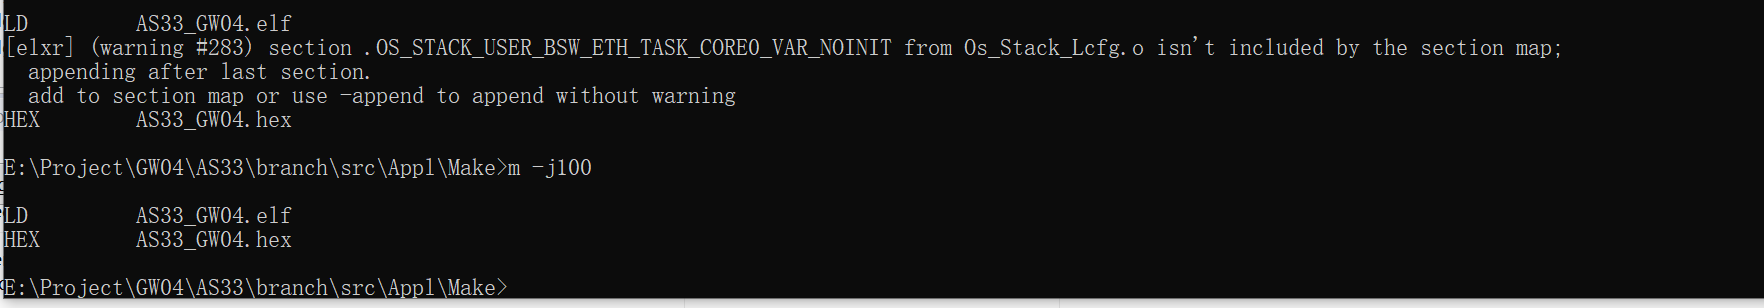
\includegraphics[scale=0.6]{pic/eth_ld_error_task.png}
    \caption{以太网 Task 代码段链接错误}
    \label{fig:ld_error_eth_task}
\end{figure}

添加新的\lstinline{Task}后,需要重新生成 \lstinline{rte os vlinkgen} 等模块。\lstinline{vlinkgen} 未生成时,报上述错误。

重要的新增生成内容如图 \ref{fig:add_task_generate_mode_code}:由于全局的 \lstinline{memmap} 文件内容修改,所以需要重新编译的文件比较多。

\begin{figure}[htbp]
    \centering
    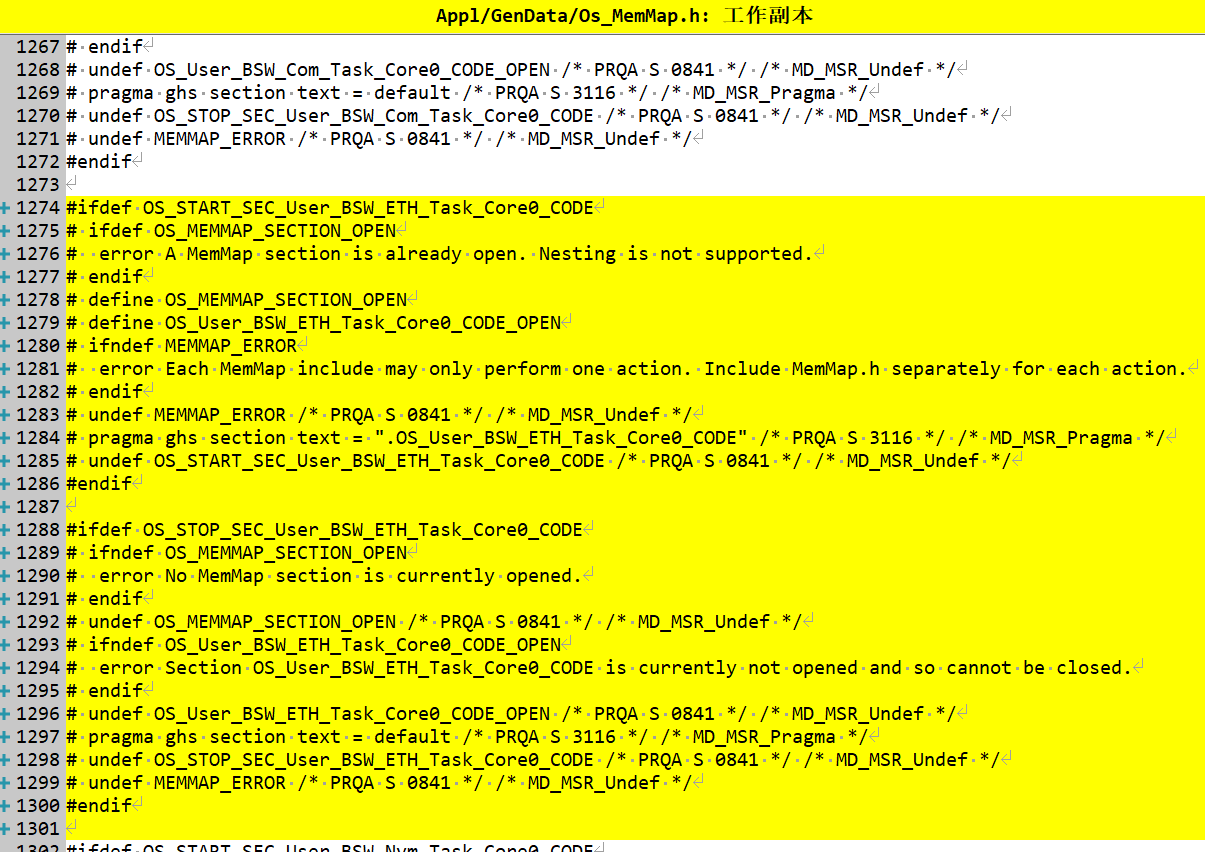
\includegraphics[scale=0.6]{pic/add_task_generate_mode_code_1.png}
    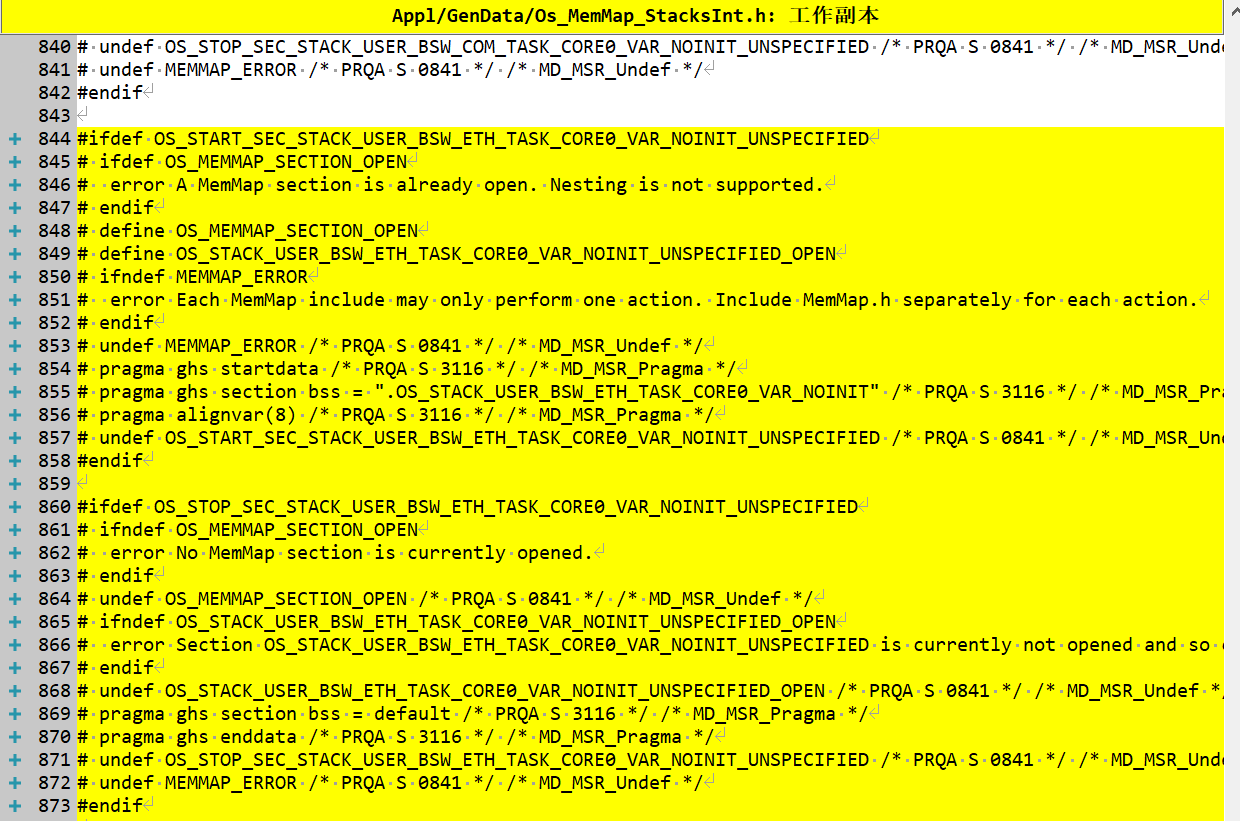
\includegraphics[scale=0.6]{pic/add_task_generate_mode_code_2.png}
    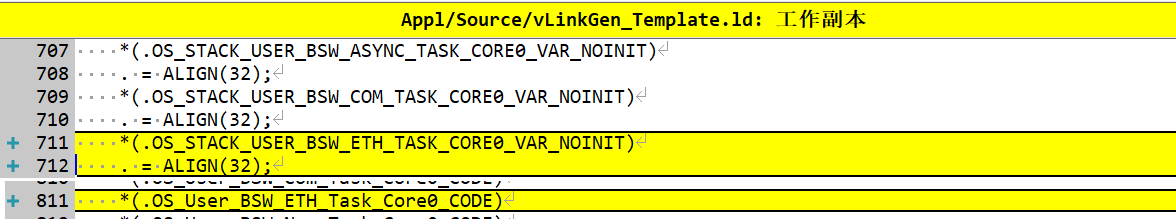
\includegraphics[scale=0.6]{pic/add_task_generate_mode_code_3.png}
    \caption{添加一个 ETH TASK 后,改变的代码}
    \label{fig:add_task_generate_mode_code}
\end{figure}

\begin{definition}[解决方案]
    当新增中断、\lstinline{Task}等内容后,需要重新生成 \lstinline{rte os vlinkgen} 等模块。
\end{definition}

\subsubsection{添加以太网中断后 \lstinline{interrupts_flash flash} 块大小溢出}\label{subsubsec:eth_ld_interrupts_flash_overflow_error}

由于对齐大小的限制,在添加以太网功能后,由于新增两个中断(\lstinline{RX TX}),导致存放中断向量表和异常向量表的 \lstinline{interrupts_flash flash} 块大小超出链接文件的大小限制。
报图 \ref{fig:eth_ld_error_interrupts_flash_overflow} 错误。此错误在链接阶段报出。

\begin{figure}[htbp]
    \centering
    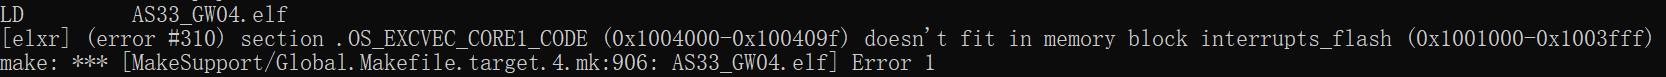
\includegraphics[scale=0.6]{pic/eth_ld_error_interrupts_flash_overflow.png}
    \caption{\lstinline{interrupts_flash flash} 块大小溢出错误}
    \label{fig:eth_ld_error_interrupts_flash_overflow}
\end{figure}

当前关于 \lstinline{interrupts_flash flash} 中存放的内容及其对齐大小如下:

\begin{lstlisting}
/* 段起始对齐大小 当前地址对齐大小 结束地址对齐大小*/
OS_INTVEC_CODE 1024
	1024 OS_INTVEC_CODE 32
OS_INTVEC_CONST 32
	OS_INTVEC_CONST 32
OS_INTVEC_CORE0_CODE 32
	4096 OS_INTVEC_CORE0_CODE 32
OS_INTVEC_CORE0_CONST 32
	4096 OS_INTVEC_CORE0_CONST 32
OS_INTVEC_CORE1_CODE 32
	4096 OS_INTVEC_CORE1_CODE 32
OS_INTVEC_CORE1_CONST 32
	4096 OS_INTVEC_CORE1_CONST 32
OS_EXCVEC_CORE0_CODE 256
	256 OS_EXCVEC_CORE0_CODE 32
OS_EXCVEC_CORE0_CONST 256
	256 OS_EXCVEC_CORE0_CONST 32	
OS_EXCVEC_CORE1_CODE 256
	256 OS_EXCVEC_CORE0_CODE 32
OS_EXCVEC_CORE1_CONST 256
	256 OS_EXCVEC_CORE0_CONST 32	

/*section name       start address   size(hex)  */
.OS_INTVEC_CODE      01001000  00002d60   // 按照段起始对齐大小对齐 1024byte 对齐
.OS_INTVEC_CONST     01003d60  00000000   //32byte 对齐

.OS_INTVEC_CORE0_CODE 01003d60  00000000  //32byte
.OS_INTVEC_CORE0_CONST 01003d60  00000000 //32byte
.OS_INTVEC_CORE1_CODE 01003d60  00000000  //32byte
.OS_INTVEC_CORE1_CONST 01003d60  00000000 //32byte
  
.OS_EXCVEC_CORE0_CODE 01003e00  000000c0  //256byte 对齐
.OS_EXCVEC_CORE0_CONST 01003f00  00000000 //256byte
.OS_EXCVEC_CORE1_CODE 01003f00  000000a0  //256byte 对齐
.OS_EXCVEC_CORE1_CONST 01004000  00000000 //256byte
\end{lstlisting}

从 \lstinline{Os_Hal_Entry_Lcfg.c} 中可以看出,\lstinline{.OS_INTVEC_CODE} 段中主要存放的是 中断向量表,即个中断处理函数的入口地址。
此外,本应放置在 \lstinline{.OS_CODE} 段的中断处理函数入口代码,也放到了\lstinline{.OS_INTVEC_CODE} 段中。导致\lstinline{.OS_INTVEC_CODE} 段占用太大。
后续再分配 \lstinline{.OS_EXCVEC_CORE0_CODE} 段和 \lstinline{.OS_EXCVEC_CORE1_CODE} 段后,\lstinline{interrupts_flash flash} 块已没有过多的空间。
添加以太网功能后,新增的两个中断符号及中断处理函数代码会继续扩大 \lstinline{.OS_INTVEC_CODE} 段的使用空间,在当前工程中,刚好超过预定义的块大小 12kB。

\begin{definition}[解决方案]
    \begin{enumerate}
        \item 在 \lstinline{Os_Hal_Entry_Lcfg.c} 中中断处理函数入口代码前手动添加 汇编级段定义语句 \lstinline{OS_HAL_OS_CODE_SECTION()}
        \item 修改各对齐大小,尽量提高空间的利用率。但减小段的对齐大小到何种程度,当前没有好的结果,实际实验结果发现,都改为32,会导致程序异常。需要进一步确定该方式。
    \end{enumerate}
\end{definition}

\subsection{开启 \lstinline{cache} 后,Switch 未能正常初始化 (AS33)}\label{subsec:desc_buffer_cache}

开启  \lstinline{cache} 后,Switch 未能正常初始化,但程序其他功能正常运行,\lstinline{Task} 正常调度。
由于初期添加以太网功能时,仅将 Switch 初始化函数放置于背景任务中,其他所有的 \lstinline{MainFunction} 均未放置到 \lstinline{Task} 调度。
所以 Swtich 不能正常初始化仅和 Switch 模块及 ETH 以太网 ENET 外设驱动模块有关。

该版本开启了 \lstinline{Data Cache},查阅 ETH 驱动模块文档,关于以太网描述符及内部使用缓存变量受 cache 的影响说明如图 \ref{fig:desc_buffer_cache}:

\begin{figure}[htbp]
    \centering
    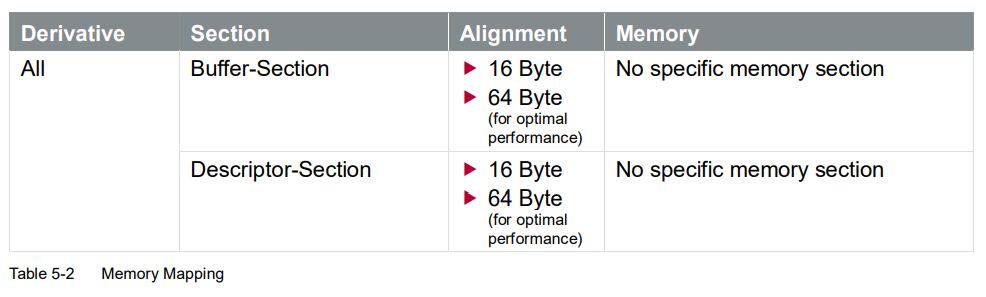
\includegraphics[scale=0.8]{pic/Snipaste_2021-11-05_13-10-08.png}
    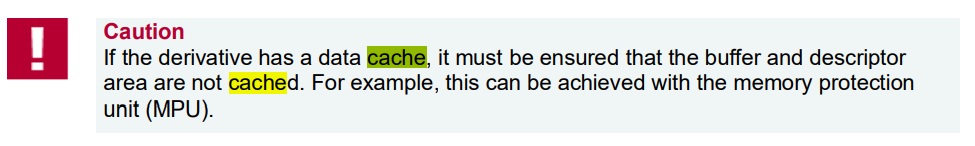
\includegraphics[scale=0.8]{pic/Snipaste_2021-11-05_13-10-26.png}
    \caption{以太网描述符、缓存存储分配及 cache 影响说明}
    \label{fig:desc_buffer_cache}
\end{figure}

因此,开启 cache 后,需要将以太网缓存及描述符变量通过 MPU 进行保护。
当前工程中,已定义 \lstinline{NONE_CACHE_DATA_RAM Block} 作为不被 cache 变量存放的区域,所以需要将以太网缓存及描述符相关变量存储的段
\lstinline{.EthRam} 放置于 \lstinline{NONE_CACHE_DATA_RAM Block}中。并在 MPU 寄存器中进行首尾 ram 地址配置。代码如下所示:


\begin{lstlisting}[language=C,style=C]
void Smpu_config(void) 
{
    /* Ensure SMPU modules are disabled */
    uint32 ces_temp = 0;
    ces_temp = REG_READ32(SMPU_0_CES0);
    ces_temp &= 0xFFFFFFFE;
    REG_WRITE32(SMPU_0_CES0, ces_temp);

    /* Create desired memory regions */
    REG_WRITE32(SMPU_0_RGD0_W0, 0x00400000);  /* Region start addr- start of SRAM */
    REG_WRITE32(SMPU_0_RGD0_W1, 0x00403fff);  /* Region end addr- end of SRAM  */
    REG_WRITE32(SMPU_0_RGD0_W2, 0xf300f000);  /* ALL masters can read/write */
    REG_WRITE32(SMPU_0_RGD0_W3, 0x00000000);  /* Region cacheable: Cache Inhibit=0*/
    REG_WRITE32(SMPU_0_RGD0_W4, 0x00000000);  /* PID not included in region eval. */
    REG_WRITE32(SMPU_0_RGD0_W5, 0x00000001);  /* Region is valid without lock */

    /* Region 1:  Shared data 16 bytes long inside SRAM, cache inhibited */
    REG_WRITE32(SMPU_0_RGD1_W0, 0x00404000);  /* Region start addr- start of SRAM */
    REG_WRITE32(SMPU_0_RGD1_W1, 0x00407fff);  /* Region end addr- end of SRAM  */
    REG_WRITE32(SMPU_0_RGD1_W2, 0xf300f000);  /* ALL masters can read/write */
    REG_WRITE32(SMPU_0_RGD1_W3, 0x00000000);  /* Region cacheable: Cache Inhibit=0*/
    REG_WRITE32(SMPU_0_RGD1_W4, 0x00000000);  /* PID not included in region eval. */
    REG_WRITE32(SMPU_0_RGD1_W5, 0x00000001);  /* Region is valid without lock */

    /* Region 2:  Shared data 16 bytes long inside SRAM, cache inhibited */
    REG_WRITE32(SMPU_0_RGD2_W0, 0x00610000);  /* Region start addr- start of SRAM */
    REG_WRITE32(SMPU_0_RGD2_W1, 0x0062ffff);  /* Region end addr- end of SRAM  */
    REG_WRITE32(SMPU_0_RGD2_W2, 0xf300f000);  /* ALL masters can read/write */
    REG_WRITE32(SMPU_0_RGD2_W3, 0x00000000);  /* Region cacheable: Cache Inhibit=0*/
    REG_WRITE32(SMPU_0_RGD2_W4, 0x00000000);  /* PID not included in region eval. */
    REG_WRITE32(SMPU_0_RGD2_W5, 0x00000001);  /* Region is valid without lock */

    /* Region 3:  Shared data 16 bytes long inside SRAM, cache inhibited */
    REG_WRITE32(SMPU_0_RGD3_W0, 0x00f80000);  /* Region start addr- start of SRAM */
    REG_WRITE32(SMPU_0_RGD3_W1, 0x00f87fff);  /* Region end addr- end of SRAM  */
    REG_WRITE32(SMPU_0_RGD3_W2, 0xf300f000);  /* ALL masters can read/write */
    REG_WRITE32(SMPU_0_RGD3_W3, 0x00000000);  /* Region cacheable: Cache Inhibit=0*/
    REG_WRITE32(SMPU_0_RGD3_W4, 0x00000000);  /* PID not included in region eval. */
    REG_WRITE32(SMPU_0_RGD3_W5, 0x00000001);  /* Region is valid without lock */

    /* Region 4:  Shared data 16 bytes long inside SRAM, cache inhibited */
    REG_WRITE32(SMPU_0_RGD4_W0, 0x00f8C000);  /* Region start addr- start of SRAM */
    REG_WRITE32(SMPU_0_RGD4_W1, 0x0157ffff);  /* Region end addr- end of SRAM  */
    REG_WRITE32(SMPU_0_RGD4_W2, 0xf300f000);  /* ALL masters can read/write */
    REG_WRITE32(SMPU_0_RGD4_W3, 0x00000000);  /* Region cacheable: Cache Inhibit=0*/
    REG_WRITE32(SMPU_0_RGD4_W4, 0x00000000);  /* PID not included in region eval. */
    REG_WRITE32(SMPU_0_RGD4_W5, 0x00000001);  /* Region is valid without lock */

    /* Region 5:  Shared data 16 bytes long inside SRAM, cache inhibited */
    REG_WRITE32(SMPU_0_RGD5_W0, 0xf0000000);  /* Region start addr- start of SRAM */
    REG_WRITE32(SMPU_0_RGD5_W1, 0xffffffff);  /* Region end addr- end of SRAM  */
    REG_WRITE32(SMPU_0_RGD5_W2, 0xf300f000);  /* ALL masters can read/write 0xf300f000*/
    REG_WRITE32(SMPU_0_RGD5_W3, 0x00000002);  /* Region cacheable: Cache Inhibit=0*/
    REG_WRITE32(SMPU_0_RGD5_W4, 0x00000000);  /* PID not included in region eval. */
    REG_WRITE32(SMPU_0_RGD5_W5, 0x00000001);  /* Region is valid without lock */

    /* SYSTEM_RAM block 可被 cache*/
    /* Region 6:  Shared data 16 bytes long inside SRAM, cache inhibited */
    REG_WRITE32(SMPU_0_RGD6_W0, 0x40000000);  /* Region start addr- start of SRAM */
    REG_WRITE32(SMPU_0_RGD6_W1, 0x4007c3ff);  /* Region end addr- end of SRAM  */
    REG_WRITE32(SMPU_0_RGD6_W2, 0xf3fcf000);  /* ALL masters can read/write- 0xc3fcf000 */
    REG_WRITE32(SMPU_0_RGD6_W3, 0x00000000);  /* Region cacheable: Cache Inhibit=0*/
    REG_WRITE32(SMPU_0_RGD6_W4, 0x00000000);  /* PID not included in region eval. */
    REG_WRITE32(SMPU_0_RGD6_W5, 0x00000001);  /* Region is valid without lock */

    /* NONE_CACHE_DATA_RAM block 不可被 cache, 包括 EthRam*/
    /* Region 7:  Shared data 16 bytes long inside SRAM, cache inhibited */
    REG_WRITE32(SMPU_0_RGD7_W0, 0x4007c400);  /* Region start addr- start of SRAM 0x4007e400*/
    REG_WRITE32(SMPU_0_RGD7_W1, 0x4007ebff);  /* Region end addr- end of SRAM  */
    REG_WRITE32(SMPU_0_RGD7_W2, 0xf3fcf000);  /* ALL masters can read/write- 0xc3fcf000 */
    REG_WRITE32(SMPU_0_RGD7_W3, 0x00000002);  /* Region cacheable: Cache Inhibit=0*/
    REG_WRITE32(SMPU_0_RGD7_W4, 0x00000000);  /* PID not included in region eval. */
    REG_WRITE32(SMPU_0_RGD7_W5, 0x00000001);  /* Region is valid without lock */

    /* Region 8:  Shared data 16 bytes long inside SRAM, cache inhibited */
    REG_WRITE32(SMPU_0_RGD8_W0, 0x4007ec00);  /* Region start addr- start of SRAM */
    REG_WRITE32(SMPU_0_RGD8_W1, 0x4007ffff);  /* Region end addr- end of SRAM  */
    REG_WRITE32(SMPU_0_RGD8_W2, 0xf3fcf000);  /* ALL masters can read/write- 0xc3fcf000 */
    REG_WRITE32(SMPU_0_RGD8_W3, 0x00000000);  /* Region cacheable: Cache Inhibit=0*/
    REG_WRITE32(SMPU_0_RGD8_W4, 0x00000000);  /* PID not included in region eval. */
    REG_WRITE32(SMPU_0_RGD8_W5, 0x00000001);  /* Region is valid without lock */

    /* Enable all SMPU regions in module */
    ces_temp = REG_READ32(SMPU_0_CES0);
    ces_temp |= 0x00000001;
    REG_WRITE32(SMPU_0_CES0, ces_temp);
    ces_temp = REG_READ32(SMPU_0_CES0);
}
\end{lstlisting}

\begin{definition}[解决方案]
    将 \lstinline{.EthRam} 放置于 \lstinline{NONE_CACHE_DATA_RAM Block}中。并在 MPU 寄存器中对 \lstinline{NONE_CACHE_DATA_RAM Block} 进行首尾 ram 地址配置。
\end{definition}